\chapter{Forth Kommunikation}
\label{chap:forthcommunication}

In diesem Kapitel wird beschrieben, wie die Entwicklungsumgebung mit dem Forth Prozess kommuniziert. Die Kommunikation mit dem Forth Prozess ist von zentraler Bedeutung, da viel der Funktionalität der Entwicklungsumgebung davon abhängt, dass die Kommunikation stabil läuft. Es wird gezeigt, wie die Kommunikation designt, implementiert und getestet wurde.

\section{Prozess Kommunikation}
Um mit dem Prozess zu kommunizieren, gibt es grundsätzlich zwei Möglichkeiten. Die erste ist ein Machine Interface zu implementieren, oder direkt mit dem Prozess kommunizieren. In folgenden Kapiteln werden die beiden Möglichkeiten kurz beschrieben.

\subsection{GDB/MI-Commands}

Eine Möglichkeit mit dem Prozess zu kommunizieren wäre, ein MachineInterface (MI) wie es für den GDB implementiert wurde, zu gebrauchen. GDB/MI ist ein Linien basiertes Maschinen orientiertes Text Interface zu dem GDB. Es wurde dazu entwickelt, damit der GDB als Debugger in ein grössers System einfacher einbindbar ist.\cite{gdb} Eine MI ähnliches Interface wäre mit grossem Aufwand verbunden, da das Interface zuerst definiert werden müsste. Dafür könnte aber viel des CDT Debugging Mechanismus verwendet werden, da der CDT Debugger auch auf dem GDB/MI basiert. Auch ist der CDT Debugger sehr kompliziert\cite{mieclipse} und es wäre ein grosser Einarbeitungsaufwand notwendig um den Forth Debugger darauf basieren zu können.\cite{mieclipse}

\subsection{Direkte Kommunikation mit dem Prozess}

Eine weitere Möglichkeit wäre, direkt die Befehle an den Prozess senden und auf Antworten warten. Dafür müsste einige Klassen implementiert werden, um das Kommunizieren zu vereinheitlichen und vereinfachen.

\subsubsection{Probleme bei der Kommunikation}

Bei der Kommunikation mit dem Prozess können einige Probleme Auftreten. Es kann sein, dass der Prozess plötzlich keine Antworten mehr gibt. Auch weiss man nicht, wie lange es dauern wird, bis der Prozess Antwort gibt. Diese Probleme müssen mit den im vorigen genannten Klassen gelöst werden.

\section{Kommunikation}

Ich habe mich dafür entschieden, die Kommunikaton nicht über ein MI ähnliches Interface zu implementieren. Der Aufwand ein solches Interface zu designen und die Einarbeitungszeit für den CDT Debugger wären zu gross. Die Kommunikation wird also direkt mit dem Prozess erfolgen. Das Design und die Implementation wird in folgenden Kapiteln besprochen.


\section{API Design}

In einem ersten Schritt wurde ein API designt, welches verwendet werden soll um die Kommunikation mit dem Prozess möglichst einfach zu halten.

\begin{figure}[H]
	\centering
		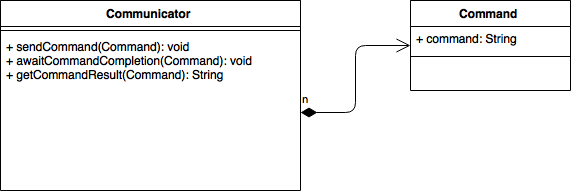
\includegraphics[scale=0.6]{forthcommunication/api.png}
		\caption{Ein erstes Design des Prozess API. Die zentrale Kommunikation geschieht über die Communicator Klasse. Es können Commands abgesetzt werden und es kann auf Resultate gewartet werden.}
		\captionsetup{margin=0cm,font={footnotesize}}
		\label{fig:api}
\end{figure}

\section{Implementierung}

Bei der Implementierung kamen dann einige Änderungen hinzu. In folgendem Klassendiagramm sind die Änderungen ersichtlich und die Klassenstruktur wird noch genauer erläutert.

\begin{sidewaysfigure}[p]

	\centering
		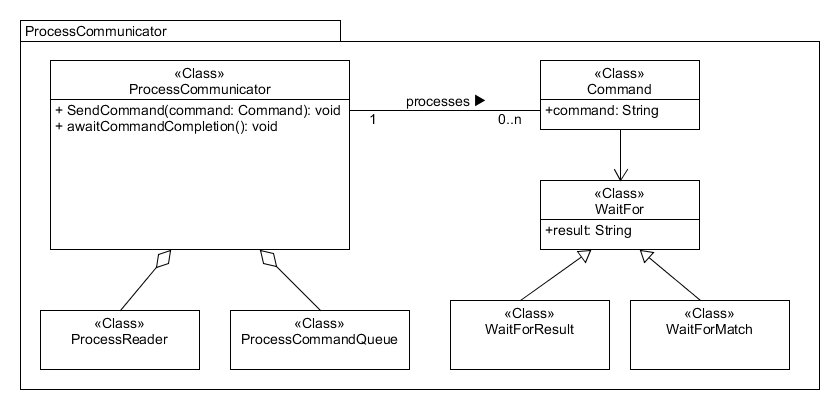
\includegraphics[scale=0.75]{forthcommunication/communicator.png}
		\caption{Klassendiagramm der.}
		\captionsetup{margin=0cm,font={footnotesize}}
		\label{fig:communicator}

\end{sidewaysfigure}

\newpage

\subsection{Klassenbeschreibung}

Über das \verb!ProcessCommunicator! API können Commands an den Prozess gesendet werden. Das API stellt blockierende und nicht blockierende Methoden für das senden von Commands an. So können Commands über die \verb!sendCommand! Funktion einen Command abschicken, ohne zu blockieren. Falls auf ein bestimmtes Resultat gewartet werden muss, kann die Funktion \verb!sendCommandAwaitResult! verwendet werden, welche den aufrufenden Thread blockiert, bis das Resultat eingetroffen ist. 

\subsubsection{ProcessCommunicator}

Der \verb!ProcessCommunicator! ist die zentrale Kommunikationsstelle. Über den \verb!ProcessCommunicator! können die \verb!Commands! gesendet werden und gleichzeitig auch auf die angeforderten Resultate warten.

\subsubsection{ProcessReader}

Der \verb!ProcessReader! ist eine verschachtelte Klasse des \verb!ProcessCommunicator!, welche als Thread im Hintergrund den Stream des Prozesses liest und verarbeitet. Der \verb!ProcessReader! notifiziert alle Threads, welche auf ein Resultat warten, falls dies eingetroffen ist.

\subsubsection{ProcessCommandQueue}

Die \verb!ProcessCommandQueue! ist eine verschachtelte Klasse des \verb!ProcessCommunicator!, welche als Thread im Hintergrund Commands verarbeitet und an den Prozess sendet. Die \verb!ProcessCommandQueue! blockiert, falls dies von einem Command spezifiert wurde. Wenn die \verb!ProcessCommandQueue! blockiert werden keine weiteren Commands mehr verarbeitet, bis das der \verb!WaitFor! Klasse spezifizierten Resultat von dem Prozess geschrieben wurde.

\subsubsection{Command}

Die \verb!Command! Klasse repräsentiert ein Command, welcher über den \verb!ProcessCommunicator! an den Prozess gesendet werden kann. In einem Command kann eine \verb!WaitFor! spezifiziert werden, fall der Command blockieren soll, bis ein Resultat von dem Prozess geliefert wird.

\newpage
\subsubsection{WaitFor}

Mit der abstrakten \verb!WaitFor! Klasse können auf Resultate des Prozesses gewartet werden. Dafür wurden verschiedene Implementationen bereitgestellt. Mit der \verb!WaitForResult! können auf String Resultate gewartet werden. Mit der \verb!WaitForMatch! Klasse kann per Regex auf ein Resultat gewartet werden. In folgendem Pseudocode wird die Funktionalität der \verb!WaitForMatch! Klasse im Zusammenhang mit dem senden eines Commands gezeigt.

\begin{verbatim}
sendCommandAwaitMatch("foo", "[1-9]")
\end{verbatim}

Der aktuelle Thread wird blockiert, bis der Prozess eine Ziffer zwischen 0 und 9 schreibt. Für das warten auf ein Resultat wurde ein Timeout von 10 Sekunden implementiert. Falls der Prozess in dieser Zeit keine Antwort gibt, wird eine \verb!CommandTimeOutException! geworfen und der \verb!ProcessCommunicator! wird heruntergefahren, das keine weiteren Commands mehr gesendet werden können.



